\let\lesson\undefined
\newcommand{\lesson}{\phantomlesson{Bài 3: Đơn vị và sai số trong vật lí}}
\chapter[Đơn vị và sai số trong vật lí]{Đơn vị và sai số trong vật lí}
\section{Lý thuyết}
\subsection{Đơn vị và thứ nguyên trong vật lí}
\subsubsection{Hệ đơn vị SI, đơn vị cơ bản và đơn vị dẫn xuất}
Tập hợp của đơn vị được gọi là hệ đơn vị. Trong khoa học có rất nhiều hệ đơn vị được sử dụng, trong đó thông dụng nhất là hệ đơn vị đo lường quốc tế SI (Système International d’unités) được xây dựng trên cơ sở của 7 đơn vị cơ bản.\\
Ngoài 7 đơn vị cơ bản, những đơn vị còn lại được gọi là đơn vị dẫn xuất. Mọi đơn vị dẫn xuất đều có thể phân tích thành các đơn vị cơ bản dựa vào mối liên hệ giữa các đại lượng tương ứng.\\
Khi số đo của đại lượng đang xem xét là một bội số hoặc ước số thập phân của mười, ta có thể sử dụng tiếp đầu ngữ như trong Bảng \ref{tab:1} ngay trước đơn vị để phần số đo được trình bày ngắn gọn.
\begin{table}[h]
	\centering
	\caption{Các đơn vị cơ bản trong hệ SI}
	\begin{tabular}{|c|c|c|c|}
		\hline
		\thead{STT} & \thead{Đơn vị} & \thead{Kí hiệu} & \thead{Đại lượng}\\
		\hline
		$1$ & \text{mét} & $\si{\meter}$ & \text{Chiều dài}\\
		\hline
		$2$ & \text{kilôgam} & $\si{\kilo\gram}$ & \text{Khối lượng}\\
		\hline
		$3$ & \text{giây} & $\si{\second}$ & \text{Thời gian}\\
		\hline
		$4$ & \text{kelvin} & $\si{\kelvin}$ & \text{Nhiệt độ}\\
		\hline
		$5$ & \text{ampe}& $\si{\ampere}$ & \text{Cường độ dòng điện}\\ 
		\hline
		$6$ & \text{mol} & $\si{\mole}$ & \text{Lượng chất}\\
		\hline
		$7$ & \text{candela} & $\si{\candela}$ & \text{Cường độ sáng}\\
		\hline
	\end{tabular}
\end{table}
\begin{table}[h]
	\centering
	\caption{Tên và kí hiệu tiếp đầu ngữ của bội số, ước số thập phân của đơn vị}
	\begin{tabular}{|c|c|c|c|c|c|}
		\hline
		\thead{Kí hiệu} & \thead{Tên đọc} & \thead{Hệ số} & \thead{Kí hiệu} & \thead{Tên đọc} & \thead{Hệ số}\\
		\hline
		Y & \text{yotta} & $10^{24}$ & \text{y} & \text{yokto} & $10^{-24}$\\
		\hline
		Z & \text{zetta} & $10^{21}$ & z & \text{zepto} & $10^{-21}$\\
		\hline
		E & \text{eta} & $10^{18}$ & \text{a} & \text{atto} & $10^{-18}$\\
		\hline
		P & \text{peta} & $10^{15}$ & f & \text{femto} & $10^{-15}$\\
		\hline
		T & \text{tera} & $10^{12}$ & p & \text{pico} & $10^{-12}$\\
		\hline
		G & \text{giga} & $10^{9}$ & n & \text{nano} & $10^{-9}$\\
		\hline
		M & \text{mega} & $10^{6}$ & \text{$\mu$} & \text{micro} & $10^{-6}$\\
		\hline
		k & \text{kilo} & $10^{3}$ & m & \text{mili} & $10^{-3}$\\
		\hline
		h & \text{hecto} & $10^{2}$ & c & \text{centi} & $10^{-2}$\\
		\hline
		da & \text{deka} & $10^{1}$ & d & \text{deci} & $10^{-1}$\\
		\hline
	\end{tabular}
	\label{tab:1}
\end{table}
\subsubsection{Thứ nguyên}
Thứ nguyên của một đại lượng là quy luật nêu lên sự phụ thuộc của đơn vị đo đại lượng đó vào các đơn vị cơ bản.
\begin{itemize}
	\item Thứ nguyên của một đại lượng $X$ được biễn diễn dưới dạng $[X]$. Thứ nguyên của một số đại lượng cơ bản thường sử dụng được thể hiện trong Bảng \ref{tab:2}.
	\item Một đại lượng vật lí có thể được biểu diễn bằng nhiều đơn vị khác nhau nhưng chỉ có một thứ nguyên duy nhất. Một số đại lượng vật lí có thể có cùng thứ nguyên.
\end{itemize}
\begin{center}
	\captionof{table}{Thứ nguyên của một số đại lượng cơ bản}
	\label{tab:2}
	\begin{tabular}{|c|c|}
		\hline
		\thead{Đại lượng cơ bản} & \thead{Thứ nguyên}\\
		\hline
		\text{[Chiều dài]} & $L$\\
		\hline
		\text{[Khối lượng]} & $M$\\
		\hline
		\text{[Thời gian]} & $T$\\
		\hline
		\text{[Cường độ dòng điện]} & $I$\\
		\hline
		\text{[Nhiệt độ]} & $K$\\
		\hline
	\end{tabular}
\end{center}
\luuy{Trong các biểu thức vật lí:
	\begin{itemize}
		\item Các số hạng trong phép cộng (hoặc trừ) phải có cùng thứ nguyên.
		\item Hai vế của một biểu thức vật lí có cùng thứ nguyên.
\end{itemize}}
\subsection{Sai số trong phép đo và cách hạn chế}
\subsubsection{Phép đo các đại lượng vật lí}
Phép đo một đại lượng vật lí là phép so sánh nó với đại lượng cùng loại được quy ước làm đơn vị.

Phép đo được phân loại thành 
\begin{itemize}
	\item \textbf{Phép đo trực tiếp} là phép xác định giá trị  một đại lượng bằng cách so sánh trực tiếp với dụng cụ đo (ví dụ như đo khối lượng bằng cân, đo nhiệt độ bằng nhiệt kế). 
	\item \textbf{Phép đo gián tiếp} là phép xác định giá trị một đại lượng thông qua một công thức liên hệ với các đại lượng được đo trực tiếp (ví dụ như đo khối lượng riêng thông qua việc xác định khối lượng và thể tích của khối vật chất).   
\end{itemize}
\subsubsection{Các loại sai số của phép đo}
\begin{center}
	\captionof{table}{Các loại sai số của phép đo}
	\begin{longtable}{|m{5em}|m{20em}|m{20em}|}
		\hline
		&\thead{Sai số hệ thống} & \thead{Sai số ngẫu nhiên}\\
		\hline
		\text{Khái niệm} & Sai số hệ thống là sai số có tính quy luật và được lặp lại ở tất cả các lần đo. Sai số hệ thống làm cho giá trị đo tăng hoặc giảm một lượng nhất định so với giá trị thực. & Sai số ngẫu nhiên là sai số xuất phát từ sai sót, phản xạ của người làm thí nghiệm hoặc từ những yếu tố ngẫu nhiên bên ngoài.\\
		\hline
		\text{Nguyên nhân} & Các dụng cụ đo các đại lượng vật lí luôn có sự sai lệch do đặc điểm và cấu tạo của dụng cụ gây ra. & Sai số này thường có nguyên nhân không rõ ràng và dẫn đến sự phân tán của các kết quả đo xung quanh một giá trị trung bình.\\
		\hline
		\text{Cách hạn chế} & Sai số hệ thống có thể được hạn chế bằng cách thường xuyên hiệu chỉnh dụng cụ đo, sử dụng thiết bị đo có độ chính xác cao. & Sai số ngẫu nhiên có thể được hạn chế bằng cách thực hiện phép đo nhiều lần và lấy giá trị trung bình để hạn chế sự phân tán của số liệu đo.\\
		\hline
	\end{longtable}
\end{center}
\luuy{Đối với một số dụng cụ đo, sai số dụng cụ thường được xác định bằng một nửa độ chia nhỏ nhất.}
\subsubsection{Cách biểu diễn sai số của phép đo}
Khi đo $n$ lần cùng một đại lượng $A$, ta thu được các giá trị khác nhau: $A_1,\, A_2,\,...,A_n$

Giá trị trung bình khi đo nhiều lần một đại lượng $A$:$$\bar{A}=\dfrac{A_1+A_2+...+A_{\text{n}}}{n},$$
là giá trị gần đúng nhất với giá trị thực của đại lượng $A$.  
\begin{itemize}
	\item Sai số tuyệt đối ứng với mỗi lần đo:
	$$\Delta A_1=|\bar{A}-A_1|;\quad\Delta A_2=|\bar{A}-A_2|;\quad\Delta A_3=|\bar{A}-A_3|;\dots; \Delta A_i=\left|\overline{A}-A_i\right|$$
	\item Sai số ngẫu nhiên là sai số tuyệt đối trung bình của $n$ lần đo:
	$$\overline{\Delta A}=\dfrac{\Delta A_1+\Delta A_2+...+\Delta A_{\textrm{n}} }{n}.$$
	\item Sai số dụng cụ $\Delta A_\text{dc}$ thường được lấy bằng nửa độ chia nhỏ nhất đối với những dụng cụ đơn giản như thước kẻ, cân bàn, bình chia độ, \dots Trong nhiều trường hợp, sai số dụng cụ thường được cung cấp chính xác bởi nhà sản xuất.
	\item Sai số tuyệt đối của phép đo cho biết phạm vi biến thiên của giá trị đo được và bằng tổng của sai số ngẫu nhiên và sai số dụng cụ:
	$$\Delta A= \overline{\Delta A}+ \Delta A_\text{dc}.$$
\end{itemize}
\subsubsection{Sai số tương đối (tỉ đối)}
Sai số tỉ đối $\delta A$ của phép đo là tỉ số giữa \bltext{sai số tuyệt đối} và \bltext{giá trị trung bình} của đại lượng cần đo, tính bằng phần trăm:
$$\delta A=\dfrac{\Delta A}{\overline A}\cdot 100\%.$$
Sai số tỉ đối càng \bltext{nhỏ} thì phép đo càng chính xác.

\subsubsection{Cách xác định sai số của phép đo gián tiếp}
Sai số của phép đo gián tiếp, được xác định theo các quy tắc:
\begin{itemize}
	\item Sai số tuyệt đối của một tổng hay hiệu thì bằng \bltext{tổng} các sai số tuyệt đối của các số hạng:\\
	Nếu $F=x\pm y\pm z \dots$ thì $\Delta F = \Delta x + \Delta y + \Delta z+\dots$.
	\item Sai số tỉ đối của một tích hay thương thì bằng \bltext{tổng} các sai số tỉ đối của các thừa số:\\ 
	Nếu $F= x^m\cdot\dfrac{y^n}{z^k}$ thì $\delta F=m\cdot\delta x+n\cdot\delta y +k\cdot\delta z$.
\end{itemize}
\textbf{Quy tắc xác định số chữ số có nghĩa (CSCN):}\\
Các chữ số có nghĩa bao gồm:
\begin{itemize}
	\item Các chữ số khác 0.
	\item Các chữ số 0 nằm giữa hai chữ số khác 0.
	\item Các chữ số 0 nằm bên phải của dấu	thập phân và một chữ số khác 0
\end{itemize}
\textit{Ví dụ:} \textbf{678} có ba chữ số có nghĩa, \textbf{6008} có bốn chữ số có nghĩa, 0,0\textbf{800} có ba chữ số có nghĩa.
\subsubsection{Cách viết kết quả đo}
$$A=\overline{A} \pm \Delta A,$$
trong đó:
\begin{itemize}
	\item $\overline A$ là giá trị trung bình,
	\item $\Delta A$ là sai số tuyệt đối. 
\end{itemize}
\section{Mục tiêu bài học - Ví dụ minh hoạ}
\begin{dang}{Tìm hiểu một số loại sai số đơn giản hay gặp khi đo các đại lượng vật lí và cách khắc phục chúng}
	\viduii{2}{
	Quan sát các hình sau và phân tích các nguyên nhân gây ra sai số của phép đo trong các trường hợp được nêu
	\begin{center}
		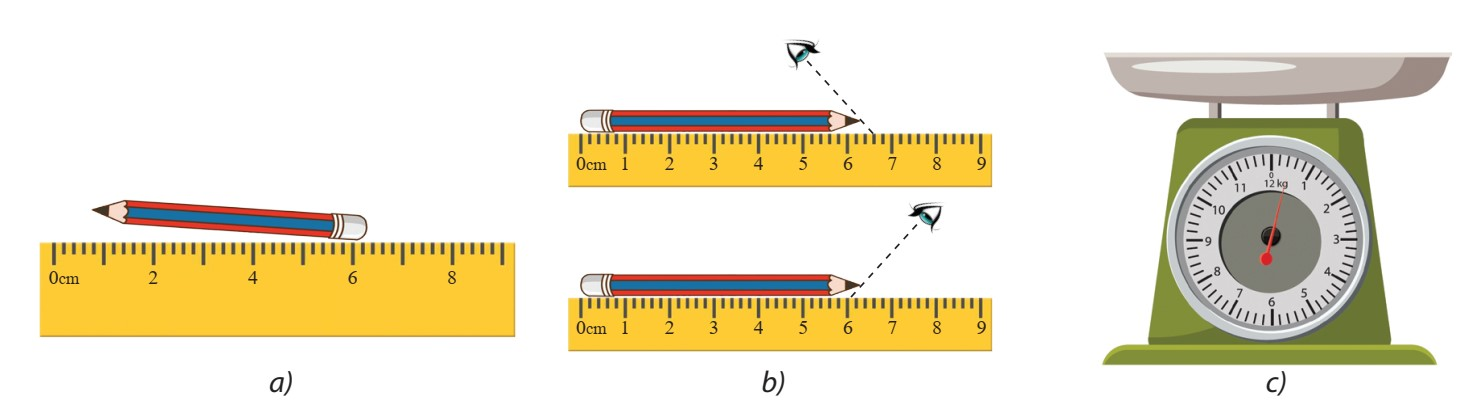
\includegraphics[width=0.7\linewidth]{../figs/VN10-2023-PH-TP003-1}
	\end{center}
}{\hide{
\begin{enumerate}[label=\alph*)]
	\item Đặt bút không dọc theo thước, đầu bút không trùng với vạch số 0.
	\item Đặt mắt sai cách, hướng nhìn không vuông góc.
	\item Kim cân chưa được hiệu chỉnh về số 0.
\end{enumerate}
}}
\end{dang}
\begin{dang}{Vận dụng mối liên hệ giữa đơn vị dẫn xuất với 7 đơn vị cơ bản của hệ SI}
	\viduii{3}
	{Để xác định quãng đường đi được $s$ của một chất điểm chuyển động thẳng đều, một bạn học sinh đã viết công thức như sau: $s=\alpha\cdot v\cdot t^2$ với $v$ và $t$ lần lượt là vận tốc và thời gian, $\alpha$ là hằng số không thứ nguyên. Dựa vào việc xác định thứ nguyên, em hãy cho biết công thức trên là đúng hay sai.
	}
{\hide{
	Thứ nguyên của các đại lượng $s$, $v$ và $t$ lần lượt là
	\begin{itemize}
		\item $\left[s\right]=L$
		\item $\left[v\right]=L\cdot T^{-1}$
		\item $\left[t\right]=T$
	\end{itemize}
Từ đó, ta thấy vế trái của công thức trên có thứ nguyên $L$ trong khi vế phải lại có thứ nguyên $L\cdot T$. Do 2 vế của công thức không cùng thứ nguyên nên bạn học sinh chưa đưa ra được công thức chính xác.\\
Dựa vào phân tích thứ nguyên, ta cần sửa lại công thức chính xác như sau:
$$s=\alpha \cdot v\cdot t$$
Trong hệ SI, $s$, $v$ và $t$ lần lượt có đơn vị là $\si{\meter}, \si{\meter\cdot\second^{-1}}, \si{\second}$.
}}
	
\end{dang}
\begin{dang}{Xác định được sai số tuyệt đối,\\ sai số tỉ đối và biểu diễn được kết quả đo}
	\viduii{3}
	{Cho bảng số liệu thể hiện kết quả đo đường kính của một viên bi thép bằng thước kẹp có sai số dụng cụ là $\SI{0.02}{\milli\meter}$. Tính sai số tuyệt đối, sai số tương đối của phép đo và biểu diễn kết quả đo có kèm theo sai số
		\begin{longtable}{|c|c|c|}
			\hline
			\thead{Lần đo} & \thead{$d \left(\si{\milli\meter}\right)$} & \thead{$\Delta d \left(\si{\milli\meter}\right)$}\\
			\hline
			1 & 6,32 & \dots\\
			\hline
			2 & 6,32 & \dots\\
			\hline
			3 & 6,32 & \dots\\
			\hline
			4 & 6,32 & \dots\\
			\hline
			5 & 6,34 & \dots\\
			\hline
			6 & 6,34 & \dots\\
			\hline
			7 & 6,32 & \dots\\
			\hline
			8 & 6,34 & \dots\\
			\hline
			9 & 6,32 & \dots\\
			\hline
			\textbf{Trung bình} & $\overline{d}=?$ & $\overline{\Delta d}=?$\\
			\hline
		\end{longtable}
	
}
{\hide{
Giá trị trung bình của đường kính viên bi:
$$\overline{d}=\dfrac{d_1+d_2+d_3+\dots+d_9}{9}\approx\SI{6.327}{\milli\meter}$$
Sai số tuyệt đối ứng với mỗi lần đo
$$\Delta d_i=\left|\overline{d}-d_i\right|$$
$$\Delta d_1=\Delta d_2=\Delta d_3=\Delta d_4=\Delta d_7=\Delta d_9=\left|\SI{6.327}{\milli\meter}-\SI{6.32}{\milli\meter}\right|=\SI{0.007}{\milli\meter}$$
$$\Delta d_5=\Delta d_6=\Delta d_8=\left|\SI{6.327}{\milli\meter}-\SI{6.34}{\milli\meter}\right|=\SI{0.013}{\milli\meter}$$
Sai số tuyệt đối trung bình của phép đo:
$$\overline{\Delta d}=\dfrac{\Delta d_1+\Delta d_2+\dots+\Delta d_9}{9}=\SI{0.009}{\milli\meter}$$
Sai số tuyệt đối của phép đo:
$$\Delta d = \overline{\Delta d}+\Delta d_\text{dc}=\SI{0.009}{\milli\meter}+\SI{0.02}{\milli\meter}=\SI{0.029}{\milli\meter}$$
Sai số tương đối của phép đo:
$$\delta d =\dfrac{\Delta d}{\overline{d}}\cdot\SI{100}{\percent}\approx\SI{0.46}{\percent}$$
Kết quả phép đo:
$$d=\overline{d}\pm\Delta d=6,273\pm\SI{0.029}{\milli\meter}.$$
}}
\end{dang}
\begin{dang}{Xác định sai số gián tiếp}
	\viduii{3}{Trong bài thực hành đo gia tốc trọng trường của Trái Đất tại phòng thí nghiệm, một học sinh đo được chiều dài của con lắc đơn $\ell= \xsi{800\pm 1}{\milli\meter}$ thì chu kì dao động là $T = \xsi{1,78\pm 0,02}{\second}$. Lấy $\pi=\SI{3.14}{}$. Biết chu kỳ của con lắc đơn tính theo công thức $T=2\pi \sqrt{\dfrac{\ell}{g}}$. Gia tốc trọng trường $g$ của Trái Đất tại phòng thí nghiệm đó là bao nhiêu?
	}
	{\hide{
		Từ công thức: $$T=2\pi \sqrt{\dfrac{\ell}{g}} \Rightarrow g=\dfrac{4\pi^2\ell}{T^2}.$$ 	
		
		Giá trị trung bình của gia tốc trọng trường: 	
		$$\overline{g}=\dfrac{4\pi^2\ell}{T^2}=\dfrac{4\pi^2\cdot \SI{3.14}{}^2\cdot \SI{0.8}{\meter}}{\left( \SI{1.78}{\second}\right)^2}=\SI{9.96}{\meter\per\second^2}.$$
		
		Sai số tuyệt đối của gia tốc trọng trường:
		\begin{align*}
			\dfrac{\Delta g}{\overline g}&= \dfrac{\Delta \ell}{\overline \ell}+ 2\dfrac{\Delta T}{\overline T}\\
			&=\dfrac{\SI{1}{\milli\meter}}{\SI{800}{\milli\meter}}+2\times\dfrac{\SI{0.02}{\second}}{\SI{1.78}{\second}}\\
			&=\SI{0.024}{}\\
			\Rightarrow\quad \Delta g&= \SI{0.024}{}\cdot \overline g\\
			&= \SI{0.24}{\meter\per\second^2}.
		\end{align*}
		
		
		
		Vậy gia tốc trọng trường của Trái Đất tại phòng thí nghiệm đó là
		$$g={\overline g } \pm \Delta g =9,96\pm\SI{0.24}{\meter\per\second^2}.$$
	}}


	\viduii{3}{Một học sinh dùng cân và đồng hồ đếm giây để đo độ cứng $k$ của lò xo. Dùng cân để cân vật nặng thu được kết quả khối lượng $m = 100 \,\text{g}$ với sai số tỉ đối là $2\%$. Gắn vật vào lò xo và kích thích cho con lắc dao động rồi dùng đồng hồ đếm giây đo thời gian của một dao động cho kết quả $T = 2\,\text{s}$ với sai số tỉ đối là $1\%$. Biết chu kỳ của con lắc lò xo tính theo công thức $T=2\pi \sqrt{m/k}$. Sai số tỉ đối của phép đo độ cứng của lò xo là bao nhiêu?
	}
	{\hide{
		Từ công thức: $$T=2\pi \sqrt{\dfrac{m}{k}} \Rightarrow k=\dfrac{4\pi^2m}{T^2}.$$	
		
		Sai số tỉ đối của độ cứng lò xo: 	
		$$\dfrac{\Delta k}{\overline k}= \dfrac{\Delta m}{\overline m}+ 2\dfrac{\Delta T}{\overline T}= 2\%+2\cdot 1\%= 4\%.$$
		
		Vậy sai số tỉ đối của phép đo độ cứng của lò xo là $4\%.$
	}}
\end{dang}
